\chapter{Experiments}
\label{chapter:experiments}

This chapter goes over some of the experiments we have conducted to evaluate the viability of Bayesian optimization. All of the cases are examples of optimizing neural networks, as that is the area of interest of this work.

We present one example from reinforcement learning, specifically the REINFORCE algorithm \citep{suttonbarto2018reinforcement}, as an example of a smaller and simpler network. This case also compares Bayesian optimization with random search. Next we show a larger experiment where we train a recurrent neural network (RNN, \cite{dlbook}), specifically a tagger, on a SIGMORPHON 2019 shared task \citep{sigmorphon2019task2}, where the network is trained on a significantly larger dataset. Lastly, we show two smaller examples, one of a tokenizer written in C++, and second a network for speech recognition.

\section{REINFORCE}

TODO: lower variance than random search?

\subsection{Comparing Priors on Kernel Parameters}
\label{section:experiments-empirical-bayes}

In this section we show the effect of setting kernel prior parameters from the data based on a simple heuristic.

TODO: empirical bayes


\section{Tuning on Multiple Treebanks Simultaneously}
\label{section:multiple-treebanks-failed}

\begin{figure}
	\begin{center}
		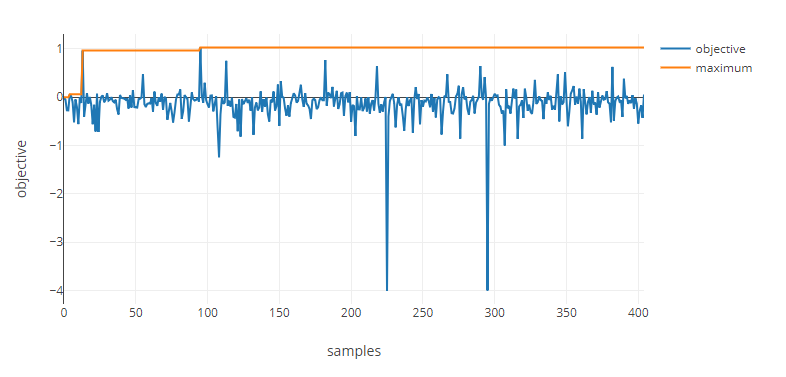
\includegraphics[width=1.0\textwidth]{images/sigmorphon-convergence.png}
		\caption{Convergence plot for a model trained on the SIGMORPHON 2019 shared task. No significant improvement over the baseline was found.}
		\label{figure:sigmorphon-convergence}
	\end{center}
\end{figure}

\begin{figure}
	\begin{center}
		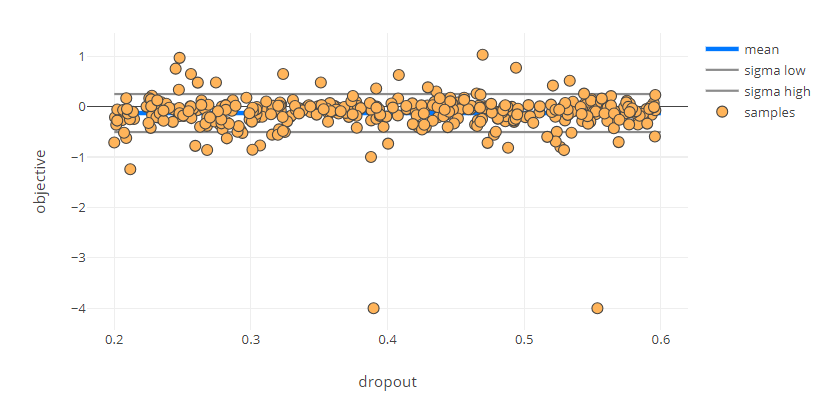
\includegraphics[width=1.0\textwidth]{images/sigmorphon-dropout.png}
		\caption{Marginal regression on the dropout hyperparameter for the SIGMORPHON 2019 shared task when training on all 105 treebanks.}
		\label{figure:sigmorphon-dropout}
	\end{center}
\end{figure}

In this larger experiment we tried to tune hyperparameters for a single model on multiple different datasets at once. Specifically, the model was trained on for the SIGMORPHON 2019 shared task 2 \citep{sigmorphon2019task2} on 105 different treebanks, most of which are different languages. Our goal was to ideally find one set of hyperparameters that would work well across all of these treebanks. Even though this experiment was not ultimately successful we still include it in the text as the problem being solved poses interesting technical challenges from the perspective of hyperparameter tuning.

As a fundamental problem of this task, each treebank is of different size, and the difficulty of different languages varies a lot. To give a few specific examples, on Tamil the model achieves around 95\% accuracy in tagging, while on Sanskrit it achieves only 65\%. This makes it nearly impossible to set the objective function to simply be the accuracy of the model, as the same value of hyperparameters could result in the objective varying by 30\%. 

We work around this problem by computing a baseline accuracy using an existing, hand tuned, model on the same task, pre-computing its score for each treebank with a fixed set of hyperparameters, and then subtracting its value from the accuracy of our tuned model. The objective function then explicitly becomes the improvement over an existing fixed model.

A second problem we had to solve was how to incorporate the 105 treebanks into the optimization procedure. Because training the model takes multiple GPU hours even for the smaller treebanks we realistically cannot perform more than a few hundred evaluations total. Instead of training the model on all treebanks for each set of hyperparameters we only train the model on one treebank for each hyperparameter configuration chosen by Bayesian optimization.

This introduces an interesting choice. In theory, we could treat the treebank as a hyperparameter treated explicitly by Bayesian optimization. As the algorithm balances the exploration-exploitation tradeoff it should be able to pick treebanks as needed to better explore the space. But because of the different sizes and difficulties of each treebank, and the inability of Bayesian optimization to treat categorical hyperparameters well, we decided to not take this approach.

Instead, we omit the treebank from the list of hyperparameters so that the optimizer has no way of modeling it, and provide it as an explicit parameter outside of the scope of the optimizer. In theory, we could also provide the optimizer with a treebank that was used with each valuation and not allow it to optimize it when choosing a next point by overriding its choice, but this approach would most likely yield sub-optimal choices by the optimizer, as the samples would be chosen based on a different criteria than what the optimizer sees. Instead, our way of completely removing the treebank parameter from the optimization process will be seen by the optimizer as noise on the output. If it were to evaluate the same hyperparameters multiple times, the evaluation itself would receive a different treebank, and the improvement over the baseline would be different. In effect this captures our desire to find a set of hyperparameters that works well across all treebanks.

Unfortunately, our experimental results did not find a significant improvement over the hyperparameters found by hand-tuning the network (see \autoref{figure:sigmorphon-convergence}). One of the reasons is that the size of the treebank affects which hyperparameter combinations result in value of the objective function. An example of using tuning the same model on a larger treebank is shown in \autoref{section:exp-cestina}.

To give a specific example, when the \emph{batch\_size} hyperparameter is set to a larger value, it will work well on a larger treebank, but the opposite is true for a smaller treebank, where a smaller \emph{batch\_size} acts as a regularizer. This means our samples at the same batch size will be spread as far as is the objective on all treebanks. Unfortunately, this spread ends up being so large that all of the hyperparameter end up having no visible trend, as no value is clearly better than the others, as shown in \autoref{figure:sigmorphon-dropout}.


\section{Tagger on a Single Treebank}
\label{section:exp-cestina}


\begin{figure}
	\begin{center}
		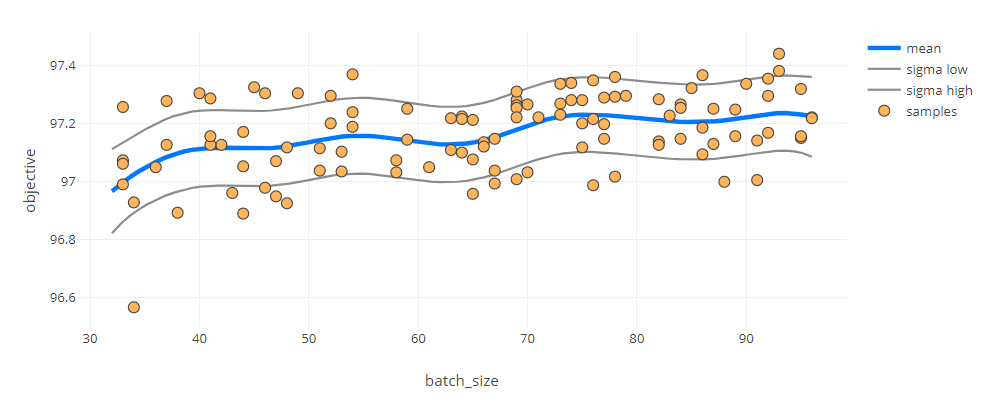
\includegraphics[width=1.0\textwidth]{images/czech-batch-size.png}
		\caption{Marginal regression on the \emph{batch\_size} hyperparameter for the SIGMORPHON 2019 shared task when training on a single Czech treebank.}
		\label{figure:czech-batch-size}
	\end{center}
\end{figure}


\begin{figure}
	\begin{center}
		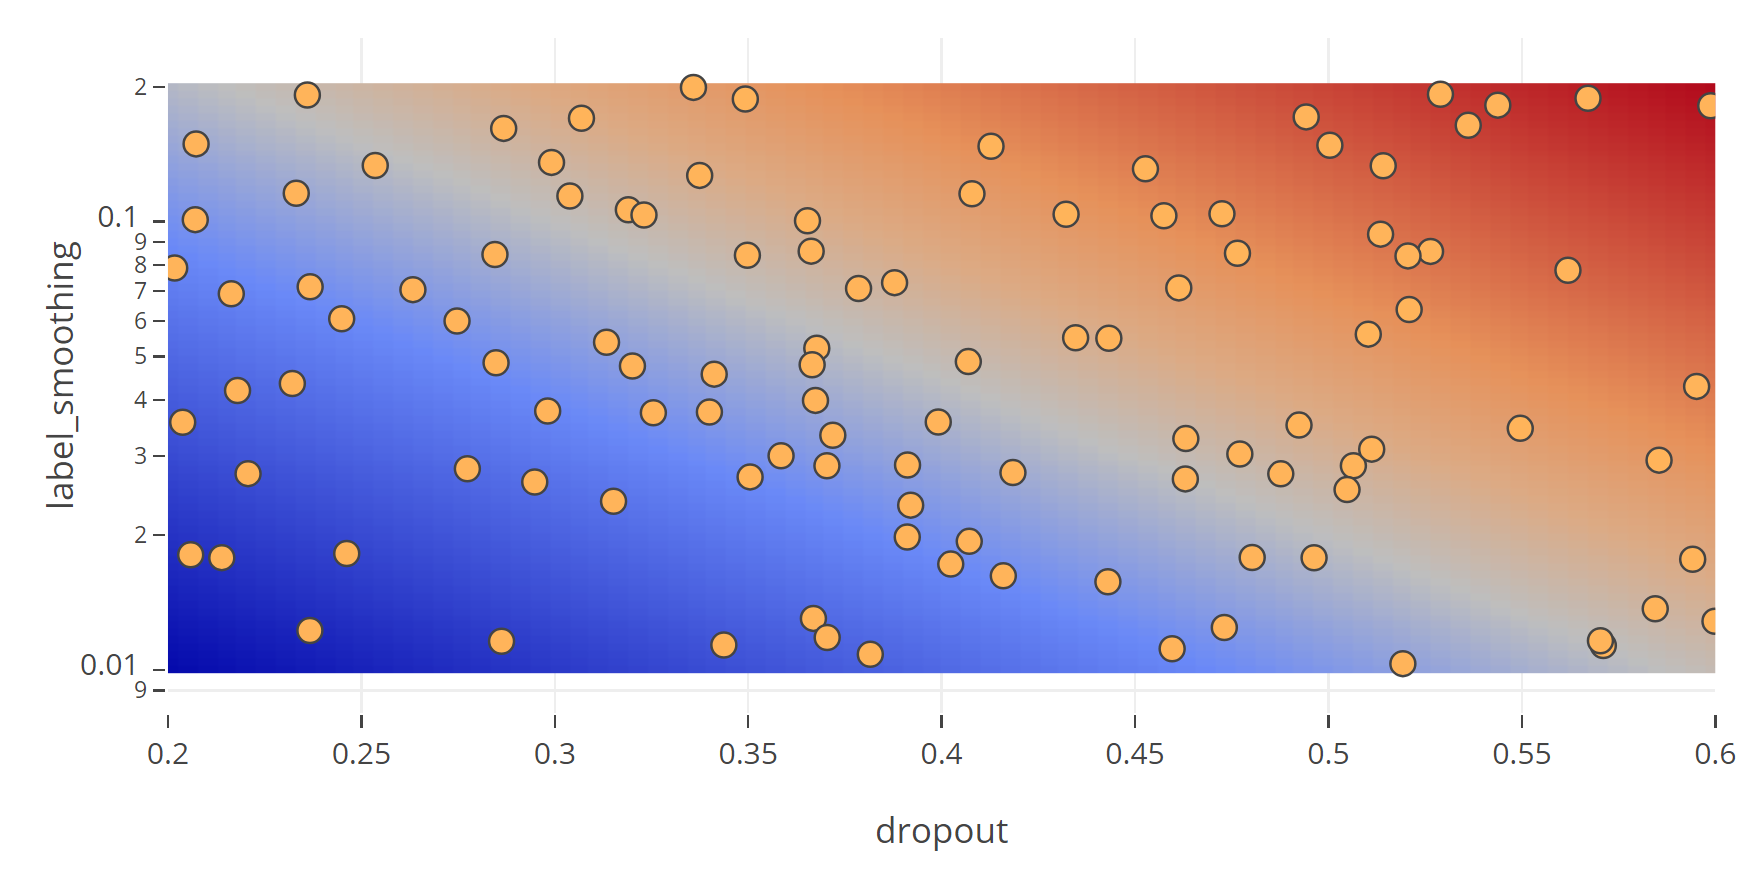
\includegraphics[width=1.0\textwidth]{images/czech-2d-marginal.png}
		\caption{Marginal regression on the \emph{label\_smoothing} and \emph{dropout} hyperparameters for the SIGMORPHON 2019 shared task when training on a single Czech treebank. A correlation between the two parameters is clearly visible, showing that setting only one of them to the correct value is not enough to achieve a high value of the objective function.}
		\label{figure:czech-2d-marginal}
	\end{center}
\end{figure}

Contrary to the experiment shown in \autoref{section:multiple-treebanks-failed} in this experiment we train the same model but only on a single treebank at a time. We tried two different treebanks, Czech and English, which are both larger. We chose the larger treebanks because they provide a more consistent evaluation metric, as the smaller ones are many orders of magnitude smaller, and pose a greater risk of overfitting even on the validation set.

While the previous experiment (see \autoref{section:multiple-treebanks-failed}) did not find any trends in the hyperparameters, the one we present here did find a clear trend in most, as shown for example in \autoref{figure:czech-batch-size}, where larger \emph{batch\_size} is better. In some cases we also found clear relationships between two hyperparameters, such as in the case of \emph{label\_smoothing} and \emph{dropout} shown in \autoref{figure:czech-2d-marginal}


\section{Other Smaller Experiments}

In this section we briefly show some interesting results from our last two experiments. First, let us show the experiment where we optimized hyperparameters of UDPipe \citep{udpipe:2017} on tokenization of Czech, English and Ancient Greek.

\begin{figure}
	\begin{center}
		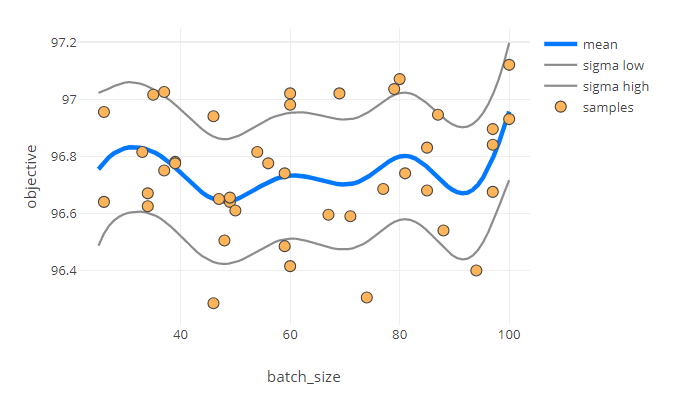
\includegraphics[width=1.0\textwidth]{images/gp-overfitting-batch-size.png}
		\caption{GP regression overfitting on the marginal distribution of \emph{batch\_size}.}
		\label{figure:gp-overfitting-batch-size}
	\end{center}
\end{figure}

Some of the interesting result in this case are the failure cases of the GP regression, particularly how it can overfit on seemingly uninformative dataset, as shown in \autoref{figure:gp-overfitting-batch-size}. These examples nicely show the high capacity of a GP which, even when we set informative priors, is able to find a surprising way to fit the data with high likelihood. Despite these problems, the Bayesian optimization approach still managed to find hyperparameter values with an objective very close to that find by an exhaustive grid search. Because of the acquisition function, even if the model overfits and picks a bad sample, it will be able to correct itself right afterwards, as the area that was previously receiving high value of acquisition function was explored.

As a result, the model still might end up wasting computation time by evaluating incorrect areas by overfitting on the data, but we have not observed it to get stuck in a local optima. Because Bayesian optimization explicitly models exploration into its decision making it quite often ends up doing a decent job of exploring most of the search space, as is visible in all of the figures.



- maly ulohy

- velka uloha

- interpretace vysledku
\\


\chapter{Conclusion}

- future work

- pribalit vysledky experimentu a jak jednoduse pustit web
